\section{Durchführung}
\label{sec:Durchführung}

\subsection{Versuchsaufbau}
\label{subsec:Versuchsaufbau}

Der Versuch wird nach \autoref{fig:Aufbau} aufgebaut.
\begin{figure}[H]
	\centering
    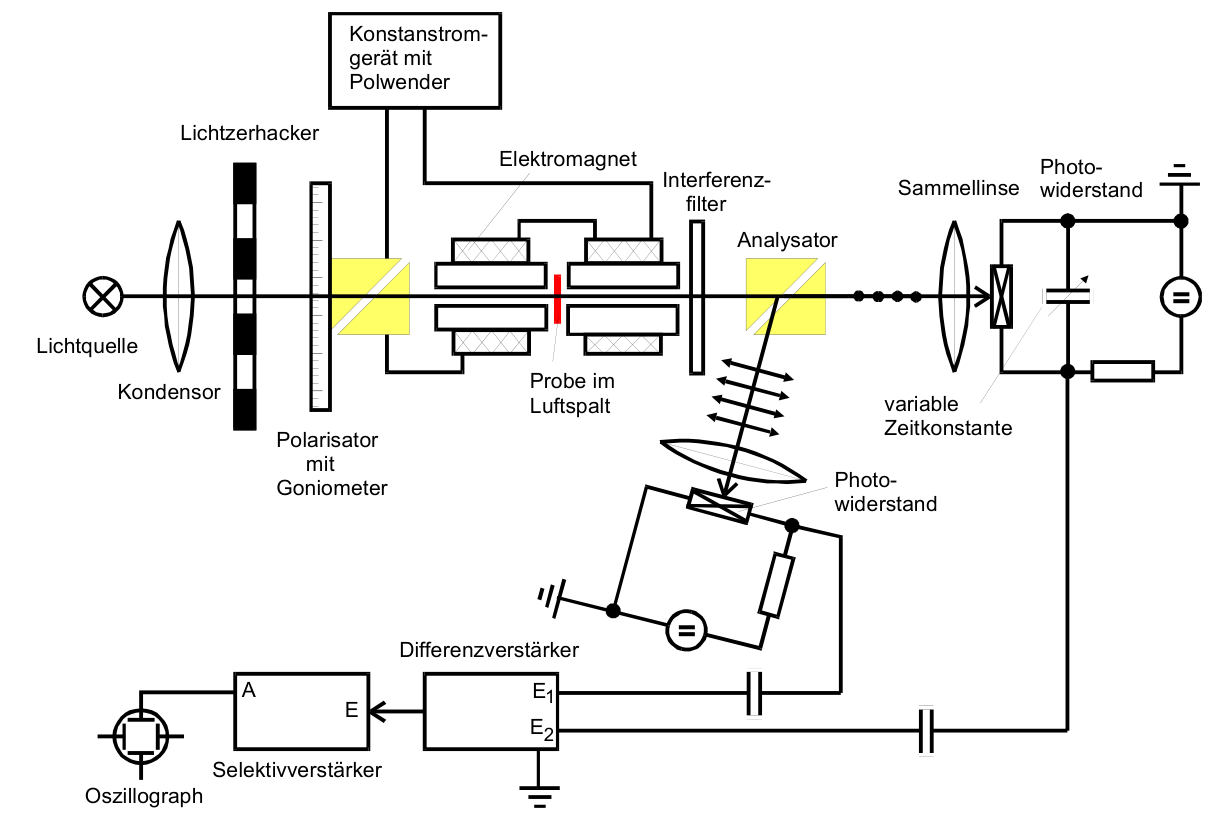
\includegraphics[width=0.6\linewidth]{data/Versuchsaufbau.png}
	\caption{Skizze des Versuchsaufbaus \cite{Anleitung46}.}
	\label{fig:Aufbau}
\end{figure}

\noindent
Als Lichtquelle wird eine Halogenlampe verwendet, dessen Lichtspektrum zum Teil im nahen Infrarotbereich liegt. Das emittierte Licht wird mithilfe einer Kondensatorlinse gebündelt. 
Danach wird der Lichtstrahl mithilfe eines Lichtzerhackers in Bündel geteilt, was das Rauschen der Photowiderstände aufgrund ihrer hohen Innenwiderstände reduziert. Der 
Lichtzerhacker ist an einen Selektivverstärker angeschlossen und verwendet dieselbe Mittenfrequenz, wie es der Lichtzerhacker tut, wodurch das Signalrauschen weiter unterdrückt wird.
Hinter dem Lichtzerhacker befindet sich ein Glan-Thomson-Prisma aus Kalkspat, das dazu genutzt wird das Licht linear zu polarisieren.
Das Licht trifft danach auf eine scheibenfömige Probe, die sich innerhalb eines Magnetfeldes befindet, dessen Magnetfeldlinien parallel zur Ausbreitungsrichtung des Lichtes 
sind. Hinter dem Elektromagneten können verschiedene Interferenzfilter geschaltet werden. Um die Rotation der Polarisationsebene messen zu können, wird der Lichtstrahl mithilfe 
eines zweiten Glan-Thomson-Prismas in zwei Teilstrahlen aufgeteilt, deren Polarisation orthogonal zueinander steht. Das Licht wird erneut durch Linsen gebündelt und die Intensität
mithilfe von Photowiderständen gemessen. Die Signale der Photowiderstände werden an einen Differenzverstärker angeschlossen, dessen Ausgang an einem Oszilloskop angezeigt wird \cite{Anleitung46}.

\subsection{Justierung der Apparatur}
\label{subsec:Justierung}

Um die Apparatur zu Justieren wird zunächst die Probe und der Interferenzfilter aus der Vorrichtung herausgenommen. Die Kondensatorlinse ist so einzustellen, dass das meiste Licht in
den vorgesehenen Lichtkanal geleitet wird.
Als nächstes muss überprüft werden, ob die Polarisationsvorrichtung funktioniert. Dazu wird das Prisma so eingestellt werden, dass die Lichtintensität von einem 
der beiden Strahlgänge vollständig verschwindet.
Nun wird der Lichtzerhacker auf \SI{450}{\hertz} eingestellt und die Mittenfrequenz beim Selektivverstärker auf denselben Wert gestellt.
Der Photowiderstand, auf den auch das Licht gestrahlt wird, wird mit dem Selektivverstärker über den Kanal ''Input'' verbunden. Der Ausgang "Resonance" 
wird an das Oszilloskop angeschlossen. Mithilfe der Frequenzstellknöpfe am Selektivverstärker wird das Signal so gewählt, das die Amplitude maximal wird.
Es ist der Gütefaktor auf den Maximalwert $Q=100$ einzustellen \cite{Anleitung46}.

\subsection{Messprogramm}
\label{subsec:Messprogramm}

Es wird nun mit einer reinen Probe des Galliumarsenid die Faraday-Rotation gemessen, indem das Glan-Thomson-Prisma bei maximaler Magnetfeldstärke so eingestellt wird,
das das Signal auf dem Oszilloskop minimal wird. Nachdem der Winkel des Prismas gemessen wurde, kann das Magnetfeld langsam heruntergedreht, umgepolt und wieder auf
den Maximalwert hochgedreht werden. Das Prisma ist erneut auf den Minimalwert einzustellen, um den Winkel abzulesen. Die Messung wird mit allen Interferenzfiltern 
wiederholt und dient später als Referenz. \newline
Das Messprogramm wird mit zwei Proben dotierten Galliumarsenids mit unterschiedlichen Dichten dotieren Materials wiederholt.
Zum Schluss wird die magnetische Flussdichte in Richtung des einfallenden Lichtes mit Hilfe einer Hall-Sonde bei maximalem Magnetfeldstrom vermessen \cite{Anleitung46}.